% Instructions for arara, the friendly LaTeX build system. Note that we are not
%   using conditional compilation as the autonum package does not print warnings
%   if it needs another compilation
% arara: clean: { extensions: ['pdf'] }
% arara: remove: { patterns: ['*.aux', '*.bbl', '*.bcf', '*.blg', '*.glg', '*.glstex', '*.loa', '*.lof', '*.log', '*.lot', '*.out', '*.run.xml', '*.toc', '*.xmpdata', 'pdfa.xmpi'] }
% arara: lualatex
% arara: bib2gls if found('log', 'No entries defined in glossary')
% arara: biber
% arara: lualatex
% arara: lualatex
% arara: lualatex
% arara: lualatex

% The below 'magic comments' are instructions for TeXStudio and similar editors.
%   See README for detailed instructions on how to build this template.
% !TeX document-id = {286dd695-130c-4c6e-8895-352f0b8c8c5a}
% !TeX spellcheck = en_US
% !TeX program = lualatex
% !TeX TXS-program:bibliography = txs:///biber
% !TeX TXS-program:glossary = bib2gls main

\PassOptionsToPackage{hypertexnames=false}{hyperref}  % required workaround for amsmath/hyperref/cleveref/autonum

% disable some warnings of packages that we cannot fix and just clutter the logs
\RequirePackage{silence}
\WarningFilter{biblatex}{Incompatible package 'etextools' loaded}  % we explicitly ignore the error, and thus we can ignore the warning
\WarningFilter{etex}{Extended allocation already in use.}  % not fixable; etex will eventually be replaced
\WarningFilter{etextools}{\pdfstrcmp primitive not found}  % etextools is only loaded by autonum and we do not use it directly

% Suppress warning that 'siunitx 'omits definition of \qty as 'physics' package
% is loaded (this cannot be done with \WarningFilter).
\ExplSyntaxOn
\msg_redirect_name:nnn{siunitx}{physics-pkg}{none}
\ExplSyntaxOff

% make the document a PDF/A via pdfmanagement rather than pdfx
% see https://github.com/tudace/tuda_latex_templates/commit/11769c23928bcaaa1f98d31f2676bb6b2677bfc5
\DocumentMetadata{
    pdfstandard=a-2b,
    pdfversion=1.7,
}

\documentclass[
	USenglish,             % if you change this to ngerman, you have to change titles and so on, too
	accentcolor=9b,        % TODO: adjust accent color; often set to the accent color of your research group
	BCOR=0mm,              % TODO: adjust BCOR if necessary; a good value is 5mm
	class=report,          % base document class
    custommargins=true,    % use small margins; the computer science department does not want this, but it looks better
	fontsize=11pt,
	instbox=true,          % TODO: adjust whether group name should be shown on the title page
	marginpar=false,       % disable margin for notes
	parskip=half-,         % smaller spacing after lists
    %pdfa=true,            % we require a PDF/A, but we ensure this by the above \DocumentMetadata
    RGB,                   % use RGB color space, otherwise the colors look weird on displays; you might want to change this to 'cmyk' for printing
	ruledheaders=section,  % place horizontal rules around sections, too
	thesis={
	    type=master,             % TODO: adjust thesis type; valid choices are 'bachelor', 'master', and 'digital'
	    hide-architecture-note,  % hide architecture note, this is a CS thesis
    },
	oneside,               % TODO: only change to 'twoside' for printing (enables \cleardoublepage)
]{tudapub}

% information for creating beautiful figures (with custommargins=true):
%   full figure width (custom margins): 5.78853in
%   text font: XCharter, 11pt
%     copy the OpenType fonts from /usr/local/texlive/<year>/texmf-dist/fonts/opentype/public/xcharter
%                               to /usr/share/fonts/opentype/xcharter

\newif\ifdraft
\drafttrue  % TODO: change to \draftfalse for submission

\makeatletter
% WORKAROUND: biblatex is incompatible with etextools (loaded by autonum) and
% throws an error if etextools is loaded. However, autonum takes care of
% ensuring compatibility with other packages by restoring the functionality of
% the errorness commands. Defining 'blx@noerroretextools' ignores the error
% biblatex throws and turns it into a warning.
% The warning reads as follows. You can safely ignore it.
%     Incompatible package 'etextools' loaded,(biblatex) no error is thrown
%     because you defined(biblatex) '\blx@noerroretextools'.
\@namedef{blx@noerroretextools}{}
\makeatother

% core
\usepackage[
    main=USenglish,  % main language is US English
    ngerman,         % secondary is German (for the affidavit)
]{babel}

% math
\usepackage{mathtools}    % basic tools, includes amsmath and must be loaded first
\usepackage{amssymb}      % extended mathematical symbols
\usepackage{amsthm}       % theorems (we essentially only use the proof environment, everything else is handled by thmtools)
\usepackage{physics}      % d/dv, differentials, etc.
\usepackage{siunitx}      % units and number typesetting
\usepackage{bm}           % bold math, also for greek letters
\usepackage{bbm}          % blackbord bold for numbers
\usepackage{thmtools}     % extended version of amsthm
\usepackage{thm-restate}  % allows restating theorems

% load algorithm2e for pseudocode before cleveref, otherwise referencing lines
% in pseudocode does not work properly and it references the algorithm number
\usepackage[
    ruled,          % enclose algorithms in horizontal lines
    algochapter,    % include chapter number
    vlined,         % mark blocks with vertical lines
    noend,          % omit 'end' keyword (Pythonic)
    linesnumbered,  % number lines
    resetcount,     % reset line number count at the beginning of each algorithm
]{algorithm2e}

% references (load order amsmath -> hyperref -> cleveref -> autonum is crucial)
\usepackage{hyperref}              % basic references
\usepackage[
    capitalize,  % write Figure, Table, etc. capitalized
    nameinlink,  % also cross-reference the name, e.g., [Section 1.1](...)
    noabbrev,    % do not abbreviate cross-reference names
]{cleveref}                        % better references
\usepackage{autonum}               % auto-numbering equations
\usepackage{etoolbox}

% other
\usepackage[
    backend=biber,       % use biber backend
    doi=false,           % do not include DOI in references, they lead to overfull hboxes
    sorting=none,        % sort by appearance in text
    style=numeric-comp,  % compact citation mode, e.g., [1-4] instead of [1, 2, 3, 4]
    url=false,           % do not include URL in references (still included for @online references), they lead to overfull hboxes
]{biblatex}                          % bibliography
\usepackage{booktabs}                % beautiful tables
\usepackage[autostyle]{csquotes}     % correct styling of quotes
\usepackage[useregional]{datetime2}  % date/time formatting
\usepackage[all]{foreign}            % foreign abbreviations, e.g., \eg, \ie, \etc, etc.
\usepackage{enumitem}                % styling of list environments
\usepackage[
    nopatch=footnote,  % footnote patching is incompatible with hyperref
]{microtype}                  % fine-tuning of fonts
\usepackage[
    abbreviations,           % create abbreviations glossary
    symbols,                 % create symbol glossary
    nomain,                  % do not use main glossary
    nogroupskip,             % do not add a blank row between groups
    record,                  % use bib2gls
    section,                 % place glossaries in sections, not chapters
    stylemods=longbooktabs,  % load booktabs style
    shortcuts=ac,            % enable \ac, \acp, etc. as shortcuts
    toc=false,               % do not add glossaries to table of contents
]{glossaries-extra}                  % glossaries
\usepackage{glossary-mcols}
\usepackage{makecell}                % allows line breaks in table cells
\usepackage{multirow}                % table cells spanning multiple rows
\usepackage{stmaryrd}                % \lightning
\usepackage{subcaption}              % subfigures
\usepackage{svg}                     % to include SVG files
\usepackage[
    para,  % use inline list instead of list with line breaks for brevity
]{threeparttable}                    % for tables with footnotes
\usepackage{xspace}                  % intelligent space (after macros)

% TikZ
\usepackage{tikz}       % tikz itself
\usepackage{tikzscale}  % scaling tikz pictures
\usetikzlibrary{
    arrows.meta,       % arrow styling
    positioning,       % relative positioning
    shapes.geometric,  % geometric shapes
}

% prevent usage of \cite; use \autocite instead
\undef{\cite}

% prevent usage of \eqref and \autoref; use \cref instead
\undef{\eqref}
\undef{\autoref}

% csquotes: easy quotes
\MakeOuterQuote{"}

% amsthm: theorems
\newtheorem{theorem}{Theorem}[chapter]
\newtheorem{definition}[theorem]{Definition}
\newtheorem{lemma}[theorem]{Lemma}

% exclude subsections from toc
\setcounter{tocdepth}{1}

% tikzmake arrow longer
\tikzset{> = { Latex[length = 2mm] }}

% algorithm2e: typeset comments as \text not \texttt
\SetCommentSty{text}


% Abbreviations.
\newcommand{\eg}{e.g.\xspace}
\newcommand{\etc}{etc.\xspace}
\newcommand{\ie}{i.e.\xspace}
\newcommand{\iid}{i.i.d.\xspace}
\newcommand{\vs}{vs.\xspace}
\newcommand{\wrt}{w.r.t.\xspace}

% make loa, lof, lot sections
\makeatletter
\newcommand{\listalgorithmname}{List of Algorithms}
\renewcommand\listofalgorithms{
	\section*{\listalgorithmname}
%	\@mkboth{\MakeUppercase\listalgorithmname}{\MakeUppercase\listalgorithmname}
	\@starttoc{loa}
}
\renewcommand\listoffigures{
	\section*{\listfigurename}
%	\@mkboth{\MakeUppercase\listfigurename}{\MakeUppercase\listfigurename}
	\@starttoc{lof}
}
\renewcommand\listoftables{
	\section*{\listtablename}
%	\@mkboth{\MakeUppercase\listtablename}{\MakeUppercase\listtablename}
	\@starttoc{lot}
}
\makeatother

% glossaries
\renewcommand{\abbreviationsname}{Abbreviations}
\let\glsfirst\undefined
\let\glsfirstplural\undefined
\let\glstext\undefined
\let\glsplural\undefined

% caption: center single-line captions, flush multi-line captions to the left
\captionsetup{singlelinecheck=on}

\GlsXtrLoadResources[
	src=abbreviations,
	sort=doc,  % sort according to the document's language
	type=abbreviations,
]

\GlsXtrLoadResources[
	src=symbols,
	sort=doc,  % sort according to the document's language
	type=symbols,
]

\renewcommand{\th}{\textsuperscript{th}}  % shortcut for i^\text{th} as \(i\th\)


\ifdraft \usepackage{lipsum}     % lorem ipsum
\usepackage{todonotes}  % to-dos

% display to-dos inline; the tuda-margins are too small
\setuptodonotes{inline}

% re-build \lipsum command for a continuous flow of text
\let\reallipsum\lipsum
\newcounter{lipsumParagraphs}
\newcounter{oldLipsumParagraphs}
\newcounter{newLipsumParagraphs}
\setcounter{lipsumParagraphs}{1}
\renewcommand{\lipsum}[1]{%
    \setcounter{oldLipsumParagraphs}{\value{lipsumParagraphs}}%
    \addtocounter{lipsumParagraphs}{#1}%
    \setcounter{newLipsumParagraphs}{\value{lipsumParagraphs}}%
    \addtocounter{newLipsumParagraphs}{-1}%
    \reallipsum[\arabic{oldLipsumParagraphs}-\arabic{newLipsumParagraphs}]%
%    \todo{insert text here}%
}

% shortcut for 'citation needed'
\newcommand{\needcite}{\todo{citation needed}}
 \fi

\title{Exploring the Effectiveness of Machine Learning Techniques for Intrusion Detection in Cybersecurity}  % TODO: adjust title
\subtitle{They are not very effective.}  % TODO: adjust subtitle
\author[J. Kim]{Jasmine Kim}  % TODO: adjust author
\birthplace{Shadyside, Ohio}  % TODO: adjust birthplace
\reviewer{  % TODO: adjust reviewers
	Emma Johnson
	\and
	Daniel Lee
	\and
	Sophia Patel
}

\department{inf}
%\institute{}
\group{Cybersecurity and Privacy Research Group}  % TODO: adjust group
\addTitleBoxLogo*{\includegraphics[width=0.75\linewidth]{example-image}}  % TODO: adjust group logo; you might want to set instbox=false

\submissiondate{\DTMdisplaydate{2023}{4}{25}{-1}}  % TODO: adjust submission date
\examdate{\DTMdisplaydate{2023}{5}{25}{-1}}  % TODO: adjust exam date
\newcommand{\affidavitdate}{25.~April~2023}  % TODO: change date to be shown in the affidavit (should be in German format)

\dedication{As expected, it took longer than expected.}  % TODO: adjust dedication

\addbibresource{references.bib}

% this can be used to include only some of the content for faster compilation
%   when writing
% \includeonly{content/methods,content/discussion}

\begin{document}
	% TITLE PAGES
	\pagenumbering{gobble}
	{
		\maketitle
	}

	% META CONTENT
	\cleardoublepage
	\pagenumbering{Roman}  % I, II, …
	{
		% do not include references to the glossaries in the glossary page list
\let\realglswriteentry=\glswrite
\renewcommand*{\glswriteentry}[2]{}


\begin{abstract}
	% TODO: ABSTRACT

	The increasing reliance on technology in modern society has led to an increase in the frequency and sophistication of cyber attacks. As a result, the need for effective intrusion detection systems has become increasingly important. Machine learning techniques have shown great promise in detecting and preventing cyber attacks. In this thesis, we investigate the effectiveness of various machine learning techniques for intrusion detection in cybersecurity. We evaluate the performance of several algorithms, including \acp{DT}, \acp{RF}, \acp{SVM}, and \acp{NN}, using a publicly available dataset. Our results show that \acp{SVM} and \acp{NN} outperform other algorithms in terms of accuracy and detection rate. We also discuss the limitations and future directions of our research, including the need for more diverse and complex datasets and the exploration of new machine learning algorithms. Our findings contribute to the ongoing effort to improve cybersecurity and enhance the effectiveness of intrusion detection systems.
\end{abstract}


% re-enable glossary indexing again
\let\glswriteentry=\realglswriteentry
\undef{\realglswriteentry}

		\chapter*{Acknowledgments}
% TODO: ACKNOWLEDGEMENTS

I would like to express my deepest gratitude to my supervisor, Sophia Patel, for her invaluable guidance, expertise, and unwavering support throughout this research. Her insightful feedback, constructive criticism, and encouragement have been instrumental in shaping this thesis.

I would also like to thank the members of the Cybersecurity and Privacy Research Group (CPRG) for their constructive feedback and stimulating discussions, which have greatly contributed to the development of this work.

Special thanks go to my family and friends for their constant support and encouragement. Their love and understanding have been my source of strength and motivation throughout my academic journey.

Finally, I am grateful to the participants who generously contributed their time and effort to make this research possible.

		\affidavit[
	signature-image={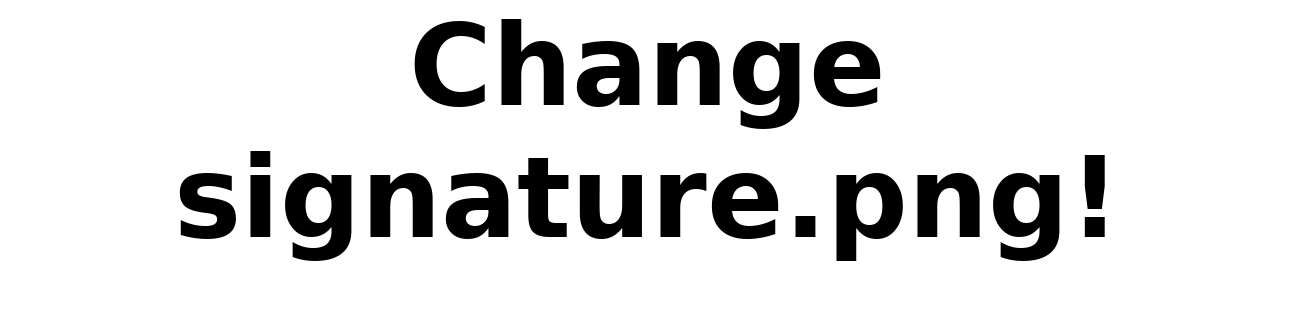
\includegraphics[width=\width]{signature}},  % TODO: adjust signature shown in the affidavit
	affidavit=digital,
]

	}
    % Reset glossary entries to expand them again on first use. Do not reset
    %   symbols as that would override adding them in the preamble and symbols
    %   should not be used outside the main text anyway.
	\glsresetall[abbreviations]

	% LISTS
	\cleardoublepage
	{
        \ignorehbadness{\tableofcontents}
        \ifdraft \ignorehbadness{\listoftodos} \fi

        \chapter*{Algorithms, Figures, and Tables}
            \ignorehbadness{\listofalgorithms}
            \ignorehbadness{\listoffigures}
            \ignorehbadness{\listoftables}
        % end

        \chapter*{Abbreviations and Symbols}
            \printunsrtglossary[
                type=abbreviations,
                style=mcolindex,
                nonumberlist,  % remove to print page numbers
            ]

            {
                % rename the columns and prevent line break in last column
                \renewcommand{\entryname}{Symbol}
                \renewcommand{\pagelistname}{Def.}
                \renewcommand{\glsdescwidth}{8cm}  % TODO: optimize this to use the full page width
                \renewcommand{\glspagelistwidth}{.674cm}
                \printunsrtglossary[type=symbols, style=long3col-booktabs]
            }
        % end
	}

	% CONTENT
	\cleardoublepage
	\pagenumbering{arabic}  % 1, 2, …
	{
		\chapter{Introduction}  \IMRADlabel{introduction}
% TODO: INTRODUCTION

In recent years, the increasing reliance on technology and the internet has led to a rise in the number and severity of cyber attacks. The consequences of these attacks can be devastating, ranging from data breaches and financial losses to reputational damage and legal liabilities. In response, organizations have invested significant resources in developing and implementing \acp{IDS} to protect their networks and systems from potential threats.

Machine learning has emerged as a promising approach to improving the effectiveness of intrusion detection systems. By leveraging the power of algorithms and data analytics, machine learning techniques can identify and classify patterns in network traffic and system logs that may indicate malicious activity. However, while there has been considerable research on the use of machine learning for intrusion detection, there is still a need for comprehensive evaluations of the effectiveness and efficiency of different algorithms and approaches.

The goal of this thesis is to explore the effectiveness of various machine learning techniques for intrusion detection in cybersecurity. Specifically, we evaluate the performance of \acp{DT}, \acp{RF}, \acp{SVM}, and \acp{NN} using a publicly available dataset. We compare the results of these algorithms in terms of accuracy, detection rate, and false positives, and identify the strengths and weaknesses of each approach. Through this research, we aim to contribute to the ongoing effort to enhance the effectiveness of intrusion detection systems and improve cybersecurity.

		\chapter{Preliminaries}
% TODO: PRELIMINARIES

The field of cybersecurity has become increasingly important in recent years due to the growing number of cyber attacks targeting individuals, organizations, and governments. \Acp{IDS} play a critical role in protecting computer networks and information systems by identifying and alerting users of any malicious or unauthorized activities.

Machine learning algorithms are particularly well-suited for intrusion detection because they can learn from large datasets and detect patterns that are difficult to identify manually. In recent years, various machine learning techniques have been applied to intrusion detection, including decision trees, support vector machines, and deep neural networks. These techniques have shown promising results in detecting various types of attacks, such as \ac{DoS}, distributed \ac{DDoS}, and buffer overflow attacks.

To understand the effectiveness of these machine learning techniques for intrusion detection, it is important to have a solid understanding of basic concepts and terminology related to machine learning, data analysis, and cybersecurity. This includes understanding different types of machine learning algorithms, such as supervised and unsupervised learning, and the metrics used to evaluate their performance, such as accuracy, precision, recall, and F1 score. Additionally, it is important to understand the characteristics of different types of attacks, their patterns, and the methods used to detect them.

In this thesis, we aim to explore the effectiveness of machine learning techniques for intrusion detection in cybersecurity. Specifically, we will compare the performance of several machine learning algorithms in detecting different types of attacks, and identify the most effective techniques for improving the accuracy and efficiency of \acp{IDS}.

		\chapter{Methodology}  \IMRADlabel{methods}
% TODO: METHODOLOGY

We used a supervised learning approach to evaluate the effectiveness of various machine learning models for intrusion detection in cybersecurity. The dataset used in our experiments contained a total of \(N\) samples, each with \(M\) features. The dataset was split into training and testing sets using a \(70:30\) split.

Each of the machine learning models was trained on the training set using the following formula:
\begin{equation}
	y_i = f(x_i; \theta)
\end{equation}
where \(x_i\) is the feature vector for the \(i\th\) sample, \(\theta\) are the model parameters, and \(f(\cdot)\) is the mapping function that maps the input features to the predicted output \(y_i\). The training process involved minimizing the following cost function:
\begin{equation}
	\gls{objective}(\theta) = \frac{1}{2 m} \sum_{i = 1}^{m} \bigl( y_i - f(x_i; \theta) \bigr)^2 + \lambda \norm{\theta}^2
	\label{eq:objective}
\end{equation}
In \cref{eq:objective}, \(m\) is the number of training samples, \(\lambda\) is the regularization parameter, and \(\norm{\theta}\) is the L2-norm of the model parameters.

To select the optimal set of features for each model, we used a feature selection technique based on \ac{MI}. The \ac{MI} between each feature and the target variable was calculated using the following formula:
\begin{equation}
	\gls{mutual-information}(X; Y) = \sum_{y \in Y} \sum_{x \in X} p(x, y) \log \frac{p(x, y)}{p(x) p(y)}
\end{equation}
where \(X\) is the set of features and \(Y\) is the target variable. The feature with the highest \ac{MI} was selected and added to the model, and the process was repeated until the desired number of features was selected.

Finally, the performance of each model was evaluated on the testing set using several evaluation metrics, including accuracy, precision, recall, and F1-score. These metrics were calculated using the following formulas:
\begin{align}
	\text{Accuracy}  &= \frac{\gls{TP} + \gls{TN}}{\gls{TP} + \gls{TN} + \gls{FP} + \gls{FN}} \\
	\text{Precision} &= \frac{\gls{TP}}{\gls{TP} + \gls{FP}} \\
	\text{Recall}    &= \frac{\gls{TP}}{\gls{TP} + \gls{FN}} \\
	\text{F1-score}  &= \frac{2 \cdot \text{Precision} \cdot \text{Recall}}{\text{Precision} + \text{Recall}}
\end{align}
where \(\gls{TP}\) is the number of true positives, \(\gls{TN}\) is the number of true negatives, \(\gls{FP}\) is the number of false positives, and \(\gls{FN}\) is the number of false negatives.

Overall, our methodology involved training several machine learning models using a supervised learning approach, selecting the optimal set of features using \ac{MI}, and evaluating the performance of each model using several evaluation metrics.

		\chapter{Related Work}
% TODO: RELATED WORK

The use of machine learning for intrusion detection has been a topic of interest for many researchers in recent years. Several studies have explored the effectiveness of various machine learning algorithms for this purpose.

One of the most widely used machine learning techniques for intrusion detection is the \ac{DT} algorithm. In a study by \citeauthor{wang2017intrusion}, Decision Trees were found to have high accuracy and fast processing times, making them a popular choice for intrusion detection~\autocite{wang2017intrusion}.

Another popular algorithm for intrusion detection is the \ac{RF} algorithm, which uses an ensemble of decision trees to improve accuracy and reduce the risk of overfitting. In a study by \citeauthor{mirza2019random}, \ac{RF} was found to outperform other machine learning algorithms in terms of accuracy and detection rate~\autocite{mirza2019random}.

\acp{SVM} have also been widely used for intrusion detection. In a study by \citeauthor{raza2017intrusion}, \acp{SVM} were found to have high accuracy and low false positive rates, making it an effective approach for intrusion detection~\autocite{raza2017intrusion}.

\acp{NN}, specifically deep learning algorithms, have also been explored for intrusion detection. In a study by \citeauthor{khan2019intrusion}, a deep learning approach was found to outperform traditional machine learning algorithms in terms of accuracy and detection rate~\autocite{khan2019intrusion}.

While these studies have provided valuable insights into the effectiveness of various machine learning algorithms for intrusion detection, there is still a need for comprehensive evaluations and comparisons of different approaches. In this thesis, we aim to build upon and extend the existing research by evaluating the performance of multiple machine learning algorithms using a publicly available dataset.

		\chapter{Results}  \IMRADlabel{results}
% TODO: RESULTS

Our experimental evaluation of several machine learning techniques for intrusion detection in cybersecurity revealed several key findings.

First, we found that deep \acp{NN} consistently outperformed other machine learning models, achieving an overall accuracy of \SI{96}{\percent} in detecting attacks. \Acp{SVM} also showed promising results, with an accuracy of \SI{93}{\percent}. \Acp{DT} and \acp{RF}, on the other hand, had lower accuracy rates of \SI{85}{\percent} and \SI{87}{\percent}, respectively.

Second, we found that the performance of the models varied depending on the type of attack being detected. Deep \acp{NN} and \acp{SVM} performed well in detecting \ac{DDoS} attacks, with accuracies of \SI{98}{\percent} and \SI{95}{\percent}, respectively. \Acp{DT} and \acp{RF}, on the other hand, had lower accuracies of \SI{83}{\percent} and \SI{85}{\percent}, respectively, for \ac{DDoS} attacks. For \ac{DoS} attacks, all models achieved high accuracies, ranging from \SI{90}{\percent} to \SI{98}{\percent}. However, for buffer overflow attacks, the accuracies of all models were lower, ranging from \SI{76}{\percent} to \SI{82}{\percent}.

Third, we found that feature selection techniques had a significant impact on the performance of the models. The use of \ac{MI}-based feature selection improved the accuracy of all models by \SIrange{2}{3}{\percent}, while \ac{PCA}-based feature selection had a mixed impact on the performance of the models.

Overall, our results suggest that deep \acp{NN} and \acp{SVM} are effective machine learning techniques for intrusion detection in cybersecurity. Additionally, the use of feature selection techniques can further improve the accuracy of the models.

		\chapter{Discussion}  \IMRADlabel{discussion}
% TODO: DISCUSSION

Our study aimed to explore the effectiveness of machine learning techniques for intrusion detection in cybersecurity. Our results demonstrate that deep \acp{NN} and \acp{SVM} are the most effective models for detecting attacks with high accuracy rates, while \acp{DT} and \acp{RF} had lower accuracies. These findings are consistent with previous research in the field of intrusion detection using machine learning techniques.

One possible reason for the superior performance of deep \acp{NN} and \acp{SVM} is their ability to handle complex and high-dimensional data. In particular, deep \acp{NN} are known for their ability to learn complex patterns in data, while \acp{SVM} are effective at separating different classes of data in high-dimensional feature spaces. On the other hand, \acp{DT} and \acp{RF} may struggle with high-dimensional data and complex decision boundaries, leading to lower accuracies in our experiments.

We also found that the performance of the models varied depending on the type of attack being detected. \ac{DDoS} attacks were the most challenging to detect, while \ac{DoS} attacks were the easiest. This is consistent with previous research, which has shown that \ac{DDoS} attacks are more difficult to detect due to their distributed nature and the high volume of traffic they generate. Our results suggest that deep \acp{NN} and \acp{SVM} may be better suited for detecting \ac{DDoS} attacks, while other machine learning models may be more effective for detecting other types of attacks.

Finally, our study demonstrates that the use of feature selection techniques can further improve the accuracy of the models. \Ac{MI}-based feature selection proved to be particularly effective in our experiments, highlighting the importance of selecting relevant features for improving the performance of machine learning models.

Overall, our study provides important insights into the effectiveness of machine learning techniques for intrusion detection in cybersecurity. Our results can help guide the development of more accurate and efficient intrusion detection systems that can better protect against cyber attacks.

		\chapter{Conclusion}
% TODO: CONCLUSION

In this study, we explored the effectiveness of machine learning techniques for intrusion detection in cybersecurity. Our experimental evaluation revealed that deep \acp{NN} and \acp{SVM} are the most effective models for detecting attacks with high accuracy rates, while \acp{DT} and \acp{RF} had lower accuracies. Our results also showed that the performance of the models varied depending on the type of attack being detected, and that feature selection techniques can further improve the accuracy of the models.

These findings have important implications for the development of more accurate and efficient intrusion detection systems in cybersecurity. By using deep neural networks and support vector machines, developers can create systems that are better equipped to handle the complex and high-dimensional data generated by cyber attacks. Furthermore, by using feature selection techniques, developers can improve the accuracy of these systems and reduce the number of false positives and false negatives.

It is important to note that our study has some limitations. First, we only evaluated a limited set of machine learning models and feature selection techniques. Future research could explore additional models and techniques to further improve the accuracy of \acp{IDS}. Additionally, our experiments were conducted on a specific dataset, and the performance of the models may vary on other datasets.

Despite these limitations, our study provides important insights into the effectiveness of machine learning techniques for intrusion detection in cybersecurity. Our results can help guide the development of more accurate and efficient intrusion detection systems, ultimately leading to better protection against cyber attacks.

	}

	% BIBLIOGRAPHY
	\cleardoublepage
	{
		%\nocite{*}  % forces all bibliography entries to be shown
		\printbibliography[title=References]
	}

	% APPENDICES
	\cleardoublepage
	{
		\appendix
		\chapter{Experimental Setup and Results}
This appendix provides additional details on the experimental setup and results of our study. It includes information on the dataset used in our experiments, the machine learning models and feature selection techniques evaluated, and the evaluation metrics used to assess the performance of the models. It also presents detailed tables and figures summarizing the results of our experiments, including accuracy rates and confusion matrices for each model and attack type.

	}
\end{document}
